% THIS FILE TAKEN FROM PANDOC DEMOS PAGE:http://johnmacfarlane.net/pandoc/demos.html,http://johnmacfarlane.net/pandoc/demo/mytemplate.tex

\documentclass[12pt, a4paper]{article}
\RequirePackage[hmargin=2cm,vmargin=2cm]{geometry}

\usepackage[T1]{fontenc}
\usepackage{lmodern}
\usepackage{amssymb,amsmath}
\usepackage{ifxetex,ifluatex}
\usepackage{fixltx2e} % provides \textsubscript

\usepackage{fontspec}
\defaultfontfeatures{Mapping=tex-text,Scale=MatchLowercase}

% Fancy HEADER
\usepackage{fancyhdr}
\pagestyle{fancy}
\pagenumbering{arabic}
\lhead{\itshape{\nouppercase{\leftmark}}}
\chead{}
\rhead{\thepage}
%\lfoot{v }
\cfoot{}
%\rfoot{\thepage}

% \usepackage{natbib}
% \bibliographystyle{abbrvnat}
% \setcitestyle{authoryear,open={(},close={)}}

\usepackage[sort&compress]{natbib}
\citestyle{nature}
\bibliographystyle{ieeetr}


\usepackage{graphicx}
% We will generate all images so they have a width \maxwidth. This means
% that they will get their normal width if they fit onto the page, but
% are scaled down if they would overflow the margins.
\makeatletter
\def\maxwidth{\ifdim\Gin@nat@width>\linewidth\linewidth
\else\Gin@nat@width\fi}
\makeatother

\let\Oldincludegraphics\includegraphics
\renewcommand{\includegraphics}[1]{\Oldincludegraphics[width=\maxwidth]{#1}}

\usepackage[rgb,dvipsnames]{xcolor}
\definecolor{ashgrey}{rgb}{0.7, 0.75, 0.71}
\definecolor{grey}{rgb}{0.5, 0.5, 0.5}

\usepackage[setpagesize=false, % page size defined by xetex
              unicode=false, % unicode breaks when used with xetex
              xetex]{hyperref}
\hypersetup{breaklinks=true,
            bookmarks=true,
            pdfauthor={},
            pdftitle={Untangling the link between traits, size and growth rate in plants},
            colorlinks=true,
            citecolor=black,
            urlcolor=grey,
            linkcolor=grey}
\setlength{\parindent}{0pt}
\setlength{\parskip}{6pt plus 2pt minus 1pt}
\setlength{\emergencystretch}{3em}  % prevent overfull lines

\usepackage{titling}

\title{Untangling the link between traits, size and growth rate in plants}

\author{
{\bf Daniel Falster} \\ \normalsize\emph{Biological Sciences, Macquarie University} \\ \url{daniel.falster@mq.edu.au}\vspace{0.1in}\\
{\bf Rich FitzJohn} \\ \normalsize\emph{Biological Sciences, Macquarie University} \\ \url{richard.fitzjohn@mq.edu.au}\vspace{0.1in}\\
{\bf Joe Wright} \\ \normalsize\emph{Center for Tropical Forest Science, Smithsonian Tropical Research Institute, Panama, Republic of Panama} \\ \url{wrightj@si.edu}\vspace{0.1in}\\ }

\date{}

\begin{document}
\thispagestyle{empty} % avoid header and footer on first page. Put after \maketitile, if using that
{\LARGE \bf \thetitle \vspace{0.2in}}

\theauthor

\section{Abstract}\label{abstract}

Plant growth is the foundation of the terrestrial biosphere, powering
food-webs, the carbon cycle and much of human
activity \citep{raupach_carbon_2010}. Plant species differ in many
functional traits, including aspects of tissue construction and energy
allocation, that drive differences in mechanical strength, biomass
partitioning, and rates of photosynthesis and tissue
turnover\citep{wright_world-wide_2004,chave_towards_2009, westoby_plant_2002}. Yet, it remains unclear how -- and even if --
such traits influence whole-plant growth, with the simple relationships
predicted by existing theory often lacking empirical
support\citep{wright_functional_2010,poorter_are_2008}. Here we
provide a new set of theoretical predictions, validated using 20 years
of growth data\citep{condit_barro_2012,kitajima_leaf_2013}, showing
that the influence of three prominent traits on growth rate is moderated
by plant size, and that the impact of size on the nature of
relationships varies among traits. We extend a widely-used theoretical
model that links growth rate in seedlings with a single leaf
trait\citep{lambers_inherent_1992,wright_cross-species_2000} to
explicitly include influences of size, light environment, and three
other prominent traits. We find the influence of leaf construction cost
(\(\phi\)) on growth is strong in small plants but weakens with size. In
contrast, the influence of stem construction cost (\(\rho\)) peaks at
intermediate sizes, while the influence of height at maturation
(\(h_m\)) strengthens with size. Our theoretical model suggests the
change in trait-growth relationships with size arises due to changes in
biomass partitioning and reproductive allocation. Moreover, we show how
traits moderate plant responses to light environment and also determine
shade tolerance, supporting diverse empirical
results\citep{ruger_functional_2012,poorter_leaf_2006}. By
disentangling the effects of plant size, light environment and traits on
growth rates, our results provide a solid theoretical foundation for
trait ecology and thus provide a platform for understanding growth
across diverse species around the world.

\section{Main text}\label{main-text}

Functional traits capture core differences in the strategies plants use
to generate and invest surplus energy\citep{wright_world-wide_2004, chave_towards_2009,westoby_plant_2002}. Data for prominent
traits now exists for many of the world's 250000 plant
species\citep{cornwell_functional_2014}; yet the effect of these traits
on growth remains poorly understood. Prominent traits such as \(\phi\)
(also known as leaf mass per area) are widely considered as indicators
of growth rate\citep{reich_world-wide_2014}, because cheaper leaf
construction should enable faster canopy
expansion\citep{blackman_compound_1919,westoby_time_2000}. Indeed,
growth rate in seedlings is strongly and negatively correlated with
\(\phi\)\citep{cornelissen_seedling_1996,wright_cross-species_2000}
(Fig. \ref{f-BCI}). Although, it has been suggested that low \(\phi\)
might also give a growth advantage in larger
plants\citep{enquist_general_2007}, an increasing number of empirical
studies have failed to detect any such
effect\citep{wright_functional_2010, @herault_functional_2011,
@poorter_are_2008}. Meanwhile, expectations on how other prominent
traits might influence growth are lacking. The growing discord between
theoretical expectation and empirical result thus indicates a strong
need for a new theoretical framework through which the influence of
traits and size on plant growth can be understood.

Here we extend a widely-used theoretical model that links growth rate in
seedlings to \(\phi\)\citep{lambers_inherent_1992, wright_cross-species_2000}, to explicitly include influences of
size, light environment, and other prominent traits. This extension
allows us to generate novel predictions on the link between four key
traits and plant demography (Table \ref{tab:predictions}). Predictions
are compared against data from both a long-term
plot\citep{condit_barro_2012} and field
experiment\citep{kitajima_leaf_2013} at Barro Colorado Island, Panama.
We use a new method to estimate species potential growth rate,
accounting for size specific effects (Fig. \ref{S-quantile_examples},
see Methods for details). This new method allowed us to extract a more
definite signal of trait effects than in previous
studies\citep{wright_functional_2010}. The results of this new analysis
(Fig. \ref{f-BCI}) align closely with our theoretical predictions (Table
\ref{tab:predictions}) showing how the effect of traits on growth
changes with plant size, with different traits exhibiting distinct
size-dependent effects.

We begin with a standard model for the amount of biomass available for
growth, \(dP / \textrm{d}t\), given by the difference between income
(total photosynthesis) and losses (respiration and turnover) within the
plant\citep{falster_influence_2011}:

\begin{equation}\label{eq:dPdt}
\underbrace{\strut \frac{dP}{\textrm{d}t}}_\textrm{net biomass production}= \underbrace{\strut Y}_\textrm{yield} \big(\underbrace{\strut \frac{m_\textrm{l}}{\phi} \, A}_\textrm{photosynthesis} - \big(\underbrace{\strut \, \frac{m_\textrm{l}}{\phi} \, r_\textrm{l} + \sum_\textrm{i=b,s,r}{m_\textrm{i} \, r_\textrm{i}}}_\textrm{respiration}\big)\big) - \big(\underbrace{\strut \sum_\textrm{i=l,b,s,r}{m_\textrm{i} \, k_\textrm{i}}}_\textrm{turnover}\big).
\end{equation}

Here, \(m,r\), and \(k\) refer to the mass, respiration rate, and
turnover rate of different tissues, denoted by subscripts \(l\)=leaves,
\(b\)=bark, \(s\)=sapwood and \(r\)=roots. \(A\) is the assimilation
rate of CO\(_2\) per leaf area and \(Y\) is yield: the fraction of
assimilated carbon fixed in biomass (the remaining fraction being lost
as growth respiration) (see Table \ref{tab:params} for units and
definitions). Photosynthesis is proportional to leaf area,
\(a_\textrm{l} = m_\textrm{l} / \phi\), while total mass of living
tissues
\(m_\textrm{t}=m_\textrm{l}+m_\textrm{b}+m_\textrm{s}+m_\textrm{r}.\)
Eq. \ref{eq:dPdt} assumes that tissues lost via turnover are replaced
before new growth occurs.

Current theory emphasises the relationship between \(\phi\) and relative
growth in mass\citep{enquist_general_2007},
\(\textrm{d}P / \textrm{d}t / m_\textrm{t}\). For seedlings, which are
young and mostly leaf, it is reasonable to ignore all turnover terms as
well as the respiration terms for non-leaf tissues. Net production then
becomes a linear function of leaf area and net photosynthesis per leaf
area (\(A_\textrm{net} = Y(A - r_\textrm{l})\)), making relative growth
rate a linear function of \(\phi\):

\begin{equation}\label{eq:RGR}
\underbrace{\strut\frac{\textrm{d}P}{\textrm{d}t}\frac{1}{m_\textrm{t}}}_\textrm{relative growth in mass}  \approx A_\textrm{net} \times \phi^{-1} \times \frac{m_\textrm{l}}{m_\textrm{t}}. \end{equation}

Although Eq. \ref{eq:RGR} captures patterns of growth in seedlings in
relation to \(\phi\)\citep{wright_cross-species_2000}, this
approximation does not directly link to other traits, or to the
variables that are routinely collected for large trees: namely plant
height (\(h\)) and stem cross-sectional area (\(a_\textrm{st}\)) or
diameter \(D\).

To model growth in either height or basal area requires we to account
not just for mass production, but also for the costs of building new
tissues, allocation to reproduction, and architectural layout. In eq.
\ref{eq:RGR}, these terms are missing, whereas in the model presented
here they are made explicit.

Mathematically, height growth can be decomposed into a product of
physiologically relevant terms\citep{falster_influence_2011}:

\begin{equation} \label{eq:dhdt}
\underbrace{\strut\frac{\textrm{d}h}{\textrm{d}t}}_\textrm{height growth rate}= \underbrace{\strut\frac{\textrm{d}h}{\textrm{d}a_\textrm{l}}}_\textrm{architecture}
\times \underbrace{\strut\frac{\textrm{d}a_\textrm{l}}{\textrm{d}m_\textrm{t}}}_\textrm{marginal leaf deployment}
\times \underbrace{\strut\frac{\textrm{d}m_\textrm{t}}{\textrm{d}P}}_\textrm{allocation to growth}
\times \underbrace{\strut\frac{\textrm{d}P}{\textrm{d}t}}_\textrm{mass production}.
\end{equation}

The first term on the right of eq \ref{eq:dhdt},
\(\textrm{d}h / \textrm{d}a_\textrm{l}\), is the growth in plant height
per unit growth in total leaf area; accounting for the architectural
strategy of the plant. Some species tend to leaf out more than grow
tall, while other species emphasise vertical
extension\citep{poorter_architecture_2006}.

The second term, \(\textrm{d}a_\textrm{l} / \textrm{d}m_\textrm{t}\),
accounts for the marginal cost of deploying an additional unit of leaf
area, including construction of the leaf itself and various support
structures. As such, \(\textrm{d}a_\textrm{l} / \textrm{d}m_\textrm{t}\)
can itself be expressed as a sum of construction costs per unit leaf
area:

\begin{equation}\label{eq:daldmt}
\frac{\textrm{d}a_\textrm{l}}{\textrm{d}m_\textrm{t}}
= \big(\phi
 + \frac{\textrm{d}m_\textrm{s}}{\textrm{d}a_\textrm{l}} + \frac{\textrm{d}m_\textrm{b}}{\textrm{d}a_\textrm{l}} + \frac{\textrm{d}m_\textrm{r}}{\textrm{d}a_\textrm{l}}\big)^{-1}.
\end{equation}

The third term in eq \ref{eq:dhdt},
\(\textrm{d}m_\textrm{t} / \textrm{d}P\), gives the fraction of net
biomass production (eq. \ref{eq:dPdt}) that is allocated to growth
rather than reproduction or storage.

In a similar way, basal area (\(a_\textrm{st}\)) increment can be
expressed as the sum of increments in sapwood, bark \& heartwood areas
(\(a_\textrm{ss}, a_\textrm{sb}, a_\textrm{sh}\) respectively):
\(\frac{\textrm{d}a_\textrm{st}}{\textrm{d}t}= \frac{\textrm{d}a_\textrm{sb}}{\textrm{d}t} + \frac{\textrm{d}a_\textrm{ss}}{\textrm{d}t} + \frac{\textrm{d}a_\textrm{sh}}{\textrm{d}t}\).
Noting that heartwood grows via turnover of sapwood, such that
\(\frac{\textrm{d}a_\textrm{sh}}{\textrm{d}t} = k_\textrm{s} a_\textrm{ss}\),
we have an equation for basal area growth that conatins many of the same
elements as eq. \ref{eq:dhdt}:

\begin{equation}\label{eq:dast}
\frac{\textrm{d}a_\textrm{st}}{\textrm{d}t}=
\left(\frac{\textrm{d}a_\textrm{ss}}{\textrm{d}a_\textrm{l}} + \frac{\textrm{d}a_\textrm{sb}}{\textrm{d}a_\textrm{l}}\right) \times
\frac{\textrm{d}a_\textrm{l}}{\textrm{d}m_\textrm{t}} \times \frac{\textrm{d}m_\textrm{t}}{\textrm{d}P} \times \frac{\textrm{d}P}{\textrm{d}t} + k_\textrm{s} a_\textrm{ss}.
\end{equation}

Diameter growth is then given by the geometric relationship between stem
diameter (\(D\)) and \(a_\textrm{st}\):

\begin{equation} \label{eq:dDdt}
\frac{\textrm{d}D}{\textrm{d}t}= \sqrt{\frac{\pi}{a_\textrm{st}}} \frac{\textrm{d}a_\textrm{st}}{\textrm{d}t}.
\end{equation}

Eqs. \ref{eq:dhdt}-\ref{eq:dDdt} are mathematically true, and must
therefore hold for any model of plant growth. To make explicit
predictions, however, requires two additional elements: 1) A specific
model describing how the various mass and area terms
(\(m_\textrm{l}, m_\textrm{s}, m_\textrm{b}, m_\textrm{r}, a_\textrm{l}, a_\textrm{s}, a_\textrm{b}\))
vary relative to one another; and 2) For any trade-offs in plant
function to be specified; this is where traits have an influence. These
two components are as follows.

To address the first of these challenges, we use a functional balance
model\citep{yokozawa_foliage_1995,falster_influence_2011} assuming
1) an allometric relation between total leaf area and plant height, and
2) a constant ratio between total leaf area and each of sapwood
cross-sectional area, bark cross-sectional area, and total root mass.
These assumptions, which are well-supported by data (Fig.
\ref{f-assumptions}), lead immediately to an allometric model for plant
size (Table \ref{tab:allometry}, see Supplementary material for
derivations). Substituting from Table \ref{tab:allometry} into eqs.
\ref{eq:dhdt}, \ref{eq:dast}, \ref{eq:dDdt} then gives an explicit model
for plant growth in relation to size.

This new growth model captures the intrinsically size-dependent nature
of plant growth (Table \ref{tab:predictions}a), recovering well-known
empirical patterns\citep{sillett_increasing_2010, king_size-related_2011}. Height growth shows a hump-shaped pattern
with size, first increasing then decreasing. This pattern results from
systematic changes in the four components of eq. \ref{eq:dhdt} with size
(Fig. \ref{f-hump}), including a strong decline in the fraction of plant
that is leaf declines with increasing size (Fig. \ref{f-mass_fraction}),
and increasing reproductive allocation. In contrast, basal-area growth
continues to increase with size\citep{sillett_increasing_2010,
@stephenson_rate_2014}, due to an increasing influence of stem
turnover. Diameter growth shows a weakly hump shaped
curve\citep{herault_functional_2011}, tapering off slightly at larger
sizes, in part because of allometric effects (eq. \ref{eq:dDdt}, but
mainly because of increased reproductive allocation in older trees
(Fig?). All growth measures decrease sharply with size when expressed as
relative growth rates\citep{iida_linking_2014}.

We now incorporate the effects of some prominent traits by embedding
explicit trade-offs within this growth model. Variation in each trait
implies benefits and costs. These affect specific elements of the growth
equations presented above (Table \ref{tab:trade-offs}).

By definition, the main effect of increasing \(\phi\) is to decrease the
marginal leaf deployment per mass (eq. \ref{eq:daldmt}) and thus reduce
growth rate. However, to fully account for the influence of \(\phi\) on
growth we must also account for the decrease in leaf turnover that
results from superior leaf construction\citep{wright_world-wide_2004}.
This is achieved by linking the turnover rate of leaf in eq.
\ref{eq:dPdt} to \(\phi\). We use an allometric scaling relationship of
the form \(k_\textrm{l}=\alpha_4 \, \phi^{-\beta_4}\), which has been
shown to describe patterns across diverse
ecosystems\citep{wright_world-wide_2004} (Fig. \ref{fS-leaf}).

Unlike eq. \ref{eq:RGR}, eqs. \ref{eq:dhdt}, \ref{eq:dast} and
\ref{eq:dDdt} predict a relationship between \(\phi\) and growth that
changes with plant size (Figs. \ref{f-BCI}, \ref{f-lma_growth_size}).
Decreasing \(\phi\) has two impacts on growth rate. First, lower
\(\phi\) increases marginal leaf deployment
(\(\textrm{d}a_\textrm{l} / \textrm{d}m_\textrm{t}\) by economising on
construction costs. Second, lower \(\phi\) decreases net production
(\(\textrm{d}P / \textrm{d}t\)), due to increased leaf turnover. Whether
lower \(\phi\) increases growth thus depends on the relative magnitude
of these two effects. When plants are small the effect on leaf
deployment rate is bigger and so decreasing \(\phi\) increases growth
rate. When plants are large, the influence of \(\phi\) on leaf
deployment rate is diminished, because the costs of building other
supportive tissues (other terms in eq. \ref{eq:daldmt}) are larger (Fig.
\ref{f-mass_fraction}). The net result is that at larger sizes, low
\(\phi\) is no longer advantageous for growth (Fig.
\ref{f-lma_growth_size}d).

As for leaf, cheaper stem construction (lower \(\rho\)) decreases the
cost of deploying a unit of leaf area, and may thereby increase growth
rates. However, the cost of cheap stem construction must also be
accounted for. However, the direct physiological trade-offs of lower
\(\rho\) are less understood than for \(\phi\). One possibility is that
lower \(\rho\) decreases mechanical strength resulting in higher
mortality\citep{chave_towards_2009,wright_functional_2010}. Under
this scenario, decreasing \(\rho\) will always provide a growth
advantage, because the costs of low \(\rho\) are not realised within the
terms of eqs. \ref{eq:dhdt} and \ref{eq:dast} (Table
\ref{tab:trade-offs}). In addition, lower \(\rho\) may increase turnover
of sapwood. Mirroring our assumptions for leaves, we let sapwood
turnover decrease with \(\rho\),
i.e.\(k_\textrm{ss}=\alpha_5 \, \rho^{-\beta_5}\), with \(\beta_5 > 1\).
Under this scenario, decreasing \(\rho\) provides an advantage in height
growth only when the benefits of low \(\rho\) outweigh the costs. This
effect is strongest at intermediate sizes. The decline in height growth
at low \(\rho\) with size is more marked than for either stem basal-area
and diameter growth, because high sapwood turnover also contributes to
this growth measure. Thus diameter growth continues, even as net
production approaches zero.

Unlike leaf and stem traits, height at maturation (\(h_m\)) moderates
growth by adjusting the amount of energy invested in growth, i.e.~the
term \(\frac{\textrm{d}m_\textrm{t}}{\textrm{d}P}\) in eqs.
\ref{eq:dhdt} and \ref{eq:dast}. Greater height at maturation (\(h_m\))
can thus lead to a growth advantage by increasing
\(\frac{\textrm{d}m_\textrm{t}}{\textrm{d}P}\) (Table
\ref{tab:predictions}). At smaller sizes, there is no differentiation
among species, because most species are focusing on growth (Fig.
\ref{f-BCI}). At larger sizes, individuals of some species are
allocating a majority of their surplus energy to growth, leaving a
strong signal in potential growth rate (Fig. \ref{f-BCI}).

Two other important predictions arise directly from linking traits to
growth rate (Table \ref{tab:predictions}c). First, traits moderate the
responsiveness of growth to changes in light environment. This response
arises simply because species with higher potential growth rate have
greater potential plasticity. Recent analyses have shown that species
with low \(rho\) increase growth more substantially with incraeses in
light\citep{ruger_functional_2012}. This is exactly the behaviour
exhibited in our model (Fig. \ref{f-growth_light}), at least for small
to intermediate sizes. At larger sizes (D=0.2m) however, the advantages
of low \(\phi\) are lost (Fig. \ref{f-growth_light}). This results also
agrees with empirical results showing that growth for species with low
\(rho\) actually decreases as size
increases\citep{ruger_functional_2012}. In contrast, growth rate tends
to increase in size for the species with highest
\(\rho\)\citep{ruger_functional_2012}.

Variation in \(\phi\) also moderates the response of growth to changes
in light, with species having the lowest \(rho\) being most responsive.
However, unlike for \(\rho\), the effect appears only for the smallest
size classes. Accordingly, empirical analyses have detected such a link
in small plants but not for plants \textgreater{} 0.01m
dbh\citep{ruger_functional_2012}.

Second, species with low \(\phi\) and low \(\rho\) are predicted to be
less shade tolerant (Fig. \ref{f-wplcp}). At low \(\phi\) (\(\rho\)),
leaf (sapwood) turnover is higher and thus a greater light income is
needed to offset these costs. As previously suggested
\citep{givnish_adaptation_1988}, shade-tolerance also decreases with
height because as size increase, the total amount of energy needed to
offset respiratory and turnover costs in the stem also increases. These
finding matches well known empirical patterns, where both \(\phi\) and
\(\rho\) have been linked to shade tolerance\citep{poorter_leaf_2006, lusk_ontogenetic_2008,osunkoya_light_1996}.

Conclusion,\ldots{}..

\begin{itemize}
\itemsep1pt\parskip0pt\parsep0pt
\item
  traits do effect growth rate, but not in the simple linear fashion
  previously anticipated.
\item
  Relationships change with size due to changes in biomass partitioning
  and reproductive allocation.
\item
  explains why LMA does not show relationship to growth among larger
  plants. Does not mean unimportant for growth, just effects
  concentrated at small sizes.
\item
  in fact, explains plasticity in LMA with size, where LMA tends to
  increase with size \citep{thomas_asymptotic_1999;
  @thomas_photosynthetic_2010}
\item
  Framework can extend to other traits (:

  \begin{itemize}
  \itemsep1pt\parskip0pt\parsep0pt
  \item
    In the current model, the only effects of the trait seed size
    (\(s\)) are to influence starting size of seedlings and fecundity of
    the mother. Seed size therefore has no direct influence on absolute
    growth. In may studies seed size has been found to be negatively
    correlated with mass-based relative growth rate of seedlings. This
    effect is recovered here because of the intrinsic decrease in RGR
    with size.
  \item
    leaf N:
  \item
    sapwood area to leaf area
  \end{itemize}
\item
  Take home: Don't look for traits as being fast or slow growth, rather
  consider traits as defining potential trajectory across sizes and
  light environments.
\end{itemize}

\section{Methods}\label{methods}

\subsection{Plant growth model}\label{plant-growth-model}

TREE

\subsection{Data analysis}\label{data-analysis}

Seedling data

\begin{itemize}
\itemsep1pt\parskip0pt\parsep0pt
\item
  about data
\item
  method for estimating growth rate
\end{itemize}

Long term plot data

\begin{itemize}
\itemsep1pt\parskip0pt\parsep0pt
\item
  about data
\item
  method for estimating growth rate
\end{itemize}

Traits

\newpage

\section{Figures}\label{figures}

\begin{figure}[htbp]
\centering
\includegraphics{figures/BCI_data.pdf}
\caption{\textbf{The relationship between traits and potential growth
rate varies with plant size.} For XXX species from tropical rain forest
in Panama, we estimated the potential growth rate of individual's in
each species at a series of diameters \(D\), indicated along right hand
side. The size of circles in each panel indicates the number of data
points used to estimate potential growth rate. Traits values were
calculated from representative individuals in each species.
\label{f-BCI}}
\end{figure}

\newpage

\begin{figure}[htbp]
\centering
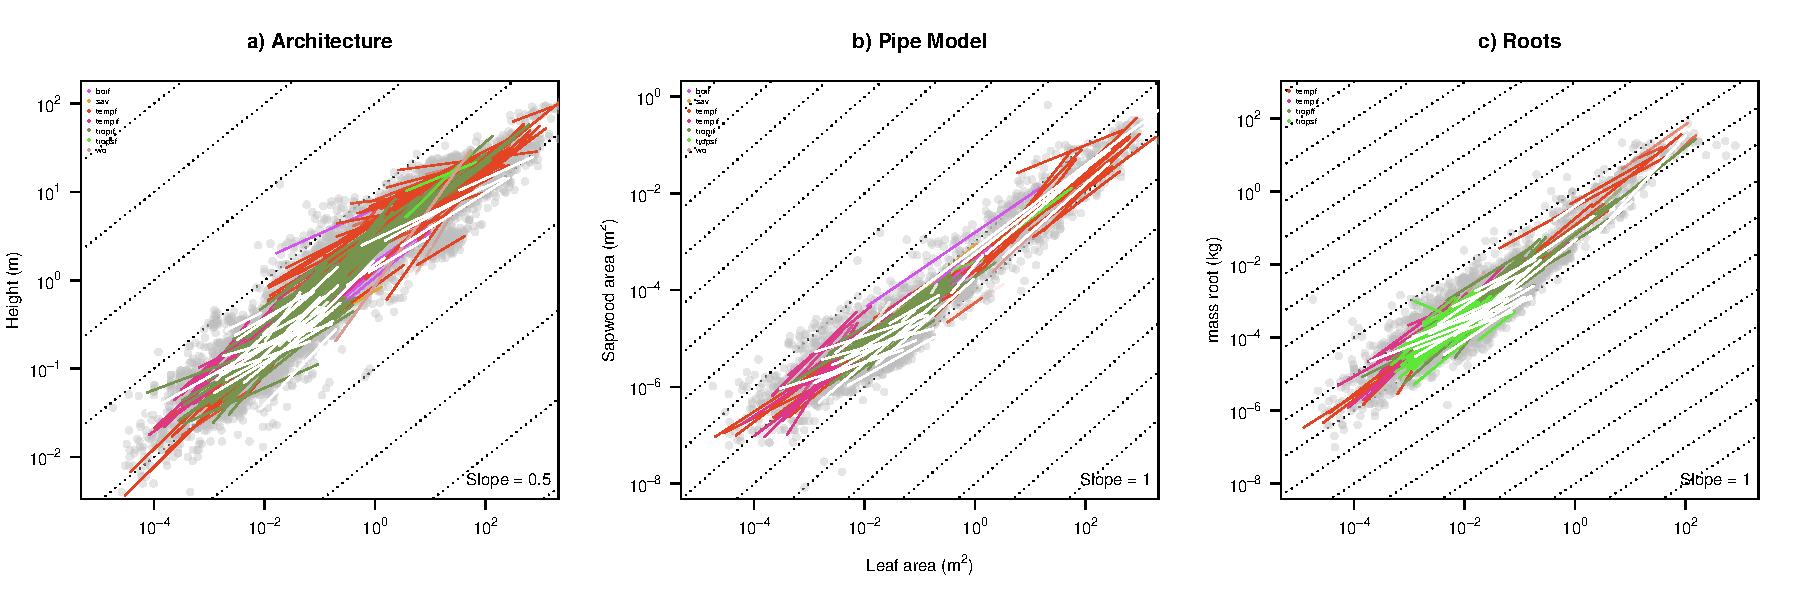
\includegraphics{figs/allometry.pdf}
\caption{\textbf{Key assumptions of a functional balance allometric
model, evaluated using global dataset.} We used the biomass and
allometry database to evaluate model assumptions about \textbf{a,}
scaling of leaf area with plant height, \textbf{b} Scaling of sapwood
area with leaf area, and \textbf{c} scaling of root mass with leaf area.
Each dot is a single plant. Lines show standardised major axis lines
fitted to data from each site, with intensity of shading adjusted
according to strength of the relationship. Colours indicate vegetation
type. Dashed black lines show values expected under functional-balance
assumption (see Supplementary text for details). \label{f-assumptions}}
\end{figure}

\newpage

\begin{figure}[htbp]
\centering
\includegraphics{figures/growth_light.pdf}
\caption{\textbf{Traits moderate the responsiveness of growth to changes
in light environment.} Panels show predicted relationship between
specific trait and diameter growth rate, for a plant of specified
diameter and under a range of shading environments.
\label{f-growth_light}}
\end{figure}

\newpage

\begin{figure}[htbp]
\centering
\includegraphics{figures/max_leaf_above.pdf}
\caption{\textbf{Low construction cost leads to shade intolerance,
because of costs of high turnover.} Panels show effect of traits on
maximum amount of shading that can be endured before net production (eq.
\ref{eq:dPdt}) reaches zero. Lines indicate relationship for plants of a
given height. \label{f-wplcp}}
\end{figure}

\newpage

\section{Tables}\label{tables}

\begin{table}[h]
\caption{Theoretical predictions on the relationship between traits and demography}

{\footnotesize
\centering
\begin{tabular}{p{4cm}p{4cm}p{2cm}p{6cm}}
\\
\multicolumn{4}{l}{\textbf{a) Intrinsic changes in demography with size}} \\ \\
\hline
Variable & Change with size & & Support \\ \hline
Height growth & strongly hump-shaped & & Fig. \ref{f-hump} \\
Diameter growth & weakly hump-shaped & & Fig. \ref{f-SI_size_dDdt}\\
Basal area growth & increases & & Fig. \ref{f-SI_size_dastdt}\\
Live mass growth & ?? & & ?? \\
ABG mass growth & increases & & ??\\
Relative growth (any) & decreases & & ??\\
Shade tolerance & decreases & & Fig. \ref{f-wplcp}\\ \\
\end{tabular}

\begin{tabular}{p{4cm}p{2.5cm}p{3.5cm}p{6cm}}
\multicolumn{4}{l}{\textbf{b) Relationship of demography to traits}} \\ \\
\hline
Variable & When small & Change with size & Support \\ \hline
\multicolumn{4}{l}{\emph{Leaf-construction cost}} \\

Height growth & negative & flattens then reverses  & Fig. \ref{f-lma_growth_size}\\
Diameter growth & negative & flattens & Fig. \ref{f-growth_light}, \ref{f-lma_growth_size}\\
Basal area growth & negative & flattens then reverses & Fig. \ref{f-lma_growth_size}\\
Live mass growth & ??  & & \\
ABG mass growth & negative & same & Fig. \ref{f-lma_growth_size} \\
Relative growth (any) & negative & weakens & Fig. \ref{f-lma_growth_size_relative}\\
Shade tolerance & positive &  strengthens & Fig. \ref{f-wplcp}\\ \\

\multicolumn{4}{l}{\emph{Wood-construction cost}} \\

Height growth & negative & strengthens  & Fig. \ref{f-rho_growth_size}\\
Diameter growth & negative & strengthens & Fig. \ref{f-growth_light}, \ref{f-rho_growth_size} \\
Basal area growth & negative & strengthens & Fig. \ref{f-rho_growth_size} \\
Live mass growth & ??  & & \\
ABG mass growth & negative & strengthens & Fig. \ref{f-rho_growth_size}\\
Relative growth (any) & negative & weakens & Fig. \ref{f-rho_growth_size_relative}\\
Shade tolerance & positive &  strengthens & Fig. \ref{f-wplcp}\\ \\

\multicolumn{4}{l}{\emph{Height at maturation}} \\
Any growth measure & none & becomes positive  & Fig. \ref{f-hmat_growth_size}\\
Relative growth (any) & none & becomes positive  & Fig. \ref{f-hmat_growth_size_relative}\\
Shade tolerance & none &  none &  \\  \\ \hline
\end{tabular}
}
\label{tab:predictions}
\end{table}

\newpage

\begin{table}[h]
\caption{Effect of traits and related trade-offs on demography}
\begin{tabular}[c]{l|ccccc|c|c|c}
\multicolumn{9}{c}{}\\ \hline
& \multicolumn{8}{c}{\textbf{Effect of trait on}}\\
& \multicolumn{5}{c|}{\textbf{Growth}} & \textbf{Mortality}& \textbf{Fecundity}& \textbf{Birth}\\
& $\frac{\textrm{d}a_\textrm{l}}{\textrm{d}m_\textrm{t}}$
& $\frac{\textrm{d}m_\textrm{t}}{\textrm{d}P}$
& $\frac{\textrm{d}P}{\textrm{d}t}$
& $\frac{\textrm{d}a_\textrm{ss}}{\textrm{d}a_\textrm{l}}$
& $\frac{1}{k_s}$ & & & $h_0$ \\\hline
\textbf{This study}&&&&&&&\\
Leaf-construction cost, $\phi$ & $\downarrow$ & $\uparrow$ & & & & & \\
Wood-construction cost, $\rho$ & $\downarrow$ &  & & & $\downarrow$ & $\downarrow$ & \\
Height at maturation, $h_m$ & &$\uparrow$ & & & & & $\downarrow$ & \\
&&&&&&&\\\hline
\textbf{Possible extensions}&&&&&&&\\
Leaf area per sapwood area, $\theta$ & $\uparrow$& & $\downarrow$ & $\downarrow$ & & &\\
Leaf-nitrogen & &$\downarrow$$\uparrow$ & & & & & \\
Seed size & & & & & & & $\downarrow$ & $\uparrow$\\ \hline
\end{tabular}
\label{tab:trade-offs}
\end{table}

\newpage

\section{Supplementary material}\label{supplementary-material}

\subsection{Derivation of a simple allometric model of plant
function}\label{derivation-of-a-simple-allometric-model-of-plant-function}

Here we describe an allometric model linking the various size dimensions
of a plant required by most ecologically realistic vegetation models
(i.e. =mass of leaves, mass of sapwood, mass of bark, mass of fine
roots) to a plant height. Table \ref{tab:allometry} provides a summary
of the derived model, while Table \ref{tab:params} provdies estimates on
key parameters.

\begin{table}[h]
\caption{Equations for an allometric growth model}
\centering

\begin{tabular}{p{5cm}p{5cm}p{5cm} }
\\ \hline
Variable & Function & Derivative\\ \hline
leaf area & $a_\textrm{l}=\alpha_1 \, h^{\beta_1}$ & $\frac{\textrm{d}h}{\textrm{d}a_\textrm{l}}= -\beta_1\big(\frac{a_\textrm{l}}{\alpha_1}\big)^{-(\beta_1+1)}$\\
leaf mass & $m_\textrm{l}=\phi \, a_\textrm{l} $ & $\frac{\textrm{d}m_\textrm{l}}{\textrm{d}a_\textrm{l}}=\phi$\\
sapwoood area & $a_\textrm{ss}=\theta^{-1} \, a_\textrm{l}$ & $\frac{\textrm{d}a_\textrm{ss}}{\textrm{d}t} =\theta^{-1} \, \frac{\textrm{d}a_\textrm{l}}{\textrm{d}t}$\\
sapwood mass&$m_\textrm{ss}=\theta^{-1} \, \rho \, \eta_c \, a_\textrm{l} \, h $ & $\frac{\textrm{d}m_\textrm{ss}}{\textrm{d}a_\textrm{l}}=\theta^{-1}\, \rho\, \eta_c\, \big( h + a_\textrm{l}\, \frac{\textrm{d}h}{\textrm{d}a_\textrm{l}} \big)$\\
bark area & $a_\textrm{sb}=b \, \theta^{-1} \, da_\textrm{l}$ & $\frac{\textrm{d}a_\textrm{sb}}{\textrm{d}t}=b \, \theta^{-1} \, \frac{\textrm{d}a_\textrm{l}}{\textrm{d}t}$\\
bark mass&$m_\textrm{b}=b\, \theta^{-1} \, \rho \, \eta_c \, a_\textrm{l} \, h $ & $\frac{\textrm{d}m_\textrm{b}}{\textrm{d}a_\textrm{l}}=b \, \theta^{-1} \, \rho \, \eta_c\big( h + a_\textrm{l} \, \frac{\textrm{d}h}{\textrm{d}A} \big)$\\
heartwood area & $a_\textrm{sh}=\int_0^t \frac{\textrm{d}a_\textrm{sh}}{\textrm{d}t}(t^\prime) \, dt^\prime$ & $\frac{\textrm{d}a_\textrm{sh}}{\textrm{d}t}=k_\textrm{s} \, a_\textrm{ss}$\\
heartwood mass & $m_\textrm{sh}=\int_0^t \frac{\textrm{d}m_\textrm{sh}}{\textrm{d}t}(t^\prime) \, dt^\prime$ & $\frac{\textrm{d}m_\textrm{sh}}{\textrm{d}t}=k_\textrm{s} \, m_\textrm{ss}$\\
root mass & $m_\textrm{r}=\alpha_3 \, a_\textrm{l}$ & $\frac{\textrm{d}m_\textrm{r}}{\textrm{d}a_\textrm{l}}= \alpha_3$ \\\hline
\end{tabular}
\label{tab:allometry}
\end{table}

\subsubsection{Leaf area}\label{leaf-area}

Based on empirically observed allometries (see main text), we assume an
allometric log-log scaling relationship between the accumulated leaf
area of a plant and its height:

\begin{equation}\label{eq:ha}
a_\textrm{l}=\alpha_1 \, h^{\beta_1}.
\end{equation}

Note, scaling relationship reversed from \citep{falster_influence_2011}.

\subsubsection{Mass of sapwood}\label{mass-of-sapwood}

We follow the model of\citep{yokozawa_foliage_1995} describing the
vertical distribution of leaf area within the crowns of individual
plants. This model can account for a variety of canopy profiles through
a single parameter \(\eta\). Setting \(\eta=1\) results in a conical
canopy, as seen in many conifers, while higher values, e.g. \(\eta=12\)
, give a top-weighted canopy profile similar to those seen among
angiosperms. Let \(S(z,h)\) be the sapwood area at height \(z\) for a
plant with top height \(h\). Following Yokozawa and Hara (1995) we
assume a relationship between \(S(z,h)\) and height such that

\begin{equation}\label{eq:crown1}
\frac{S(z,h)}{S(0,h)}= \big(1-\big(\frac{z}{h}\big)^\eta\big)^2.
\end{equation}

We also assume that each unit of sapwood area supports a fixed area of
leaf (the pipe model, \citep{shinozaki_quantitative_1964}), so that the total
canopy area of a plant relates to basal sapwood area \(S(0,h)\):

\begin{equation}\label{eq:crown2}
\frac{m_\textrm{l}}{\phi}= \theta \, S(0,h).
\end{equation}

Integrating \(S(z,h)\) gives a solution for the total mass of sapwood in
the plant:

\begin{equation}\label{eq:ms1}
m_\textrm{s}=\rho \, \int_0^h \, S(z,h) \, \textrm{d}z= \rho \, S(0,h) \, h \, \eta_c, \end{equation}

where
\(\eta_c=1-\frac{2}{1+\eta} + \frac{1}{1+2\eta}\)\citep{yokozawa_foliage_1995}.
Substituting from eq. \ref{eq:crown2} into eq. \ref{eq:ms1} gives an
expression for sapwood mass as a function leaf area and height:

\begin{equation}\label{eq:ms2}
m_\textrm{s}=\rho \, \eta_c \, \theta^{-1} \, a_\textrm{l} \, h.
\end{equation}

\subsubsection{Bark mass}\label{bark-mass}

Bark and phloem tissue are modelled using an analogue of the pipe model,
leading to a similar equation as that for sapwood mass (eq.
\ref{eq:ms2}). Cross sectional-area of bark per unit leaf area is
assumed to be a constant fraction \(b\) of sapwood area per unit leaf
area such that

\begin{equation}\label{eq:mb}
m_\textrm{b}=b m_\textrm{s}.
\end{equation}

\subsubsection{Root mass}\label{root-mass}

Also consistent with pipe-model assumption, we assume a fixed ratio of
root mass per unit leaf area

\begin{equation}\label{eq:mr}
m_\textrm{r}=\alpha_3 \, a_\textrm{l}.
\end{equation}

Even though nitrogen and water uptake are not modelled explicitly,
imposing a fixed ratio of root mass to leaf area ensures that
approximate costs of root production are included in calculations of
carbon budget.

\newpage

\begin{table}[h]
\caption{Model parameters}
\centering

\include{figures/table-pars}

\label{tab:params}
\end{table}

\subsection{Trait values maximising height
growth}\label{trait-values-maximising-height-growth}

We want to find the trait values maximising growth rate, \(G\). To make
the analysis more tractible, we will focus on height growth rate and
assume we are dealing with a plant of given height where 100\% of
available energy is allocated to growth. From eq. \ref{eq:dhdt}, we thus
have

\begin{equation} \label{eq:G1}
G = \frac{\textrm{d}h}{\textrm{d}t} = \frac{\textrm{d}h}{\textrm{d}a_\textrm{l}}
\times \frac{\textrm{d}a_\textrm{l}}{\textrm{d}m_\textrm{t}}
\times \frac{\textrm{d}m_\textrm{t}} {\textrm{d}P}
\times \frac{\textrm{d}P}{\textrm{d}t}.
\end{equation}

Maximising \(G\) is equivalent to solving for trait values \(x\) giving
\(\partial G /\partial x = 0\). Noting that traits do not influence
\(\frac{\textrm{d}h} {\textrm{d}a_\textrm{l}}\), and by assumption
\(\frac{\textrm{d}m_\textrm{t}}{\textrm{d}P}=1\), we thus have

\begin{equation} \label{eq:G2}
G =  c_1   \left(\frac{\textrm{d}a_\textrm{l}} {\textrm{d}m_\textrm{t}}  \frac{ \textrm{d}P} {\textrm{d}t} \right),
\end{equation}

where \(c_1 = \frac{\textrm{d}h}{\textrm{d}a_\textrm{l}}\). Eq.
\ref{eq:G2} is a product of the form \(Y = W(x) \times Z(x)\). For,
equations of this type, a solution to \(\partial{Y}/\partial{x} =0\) is
given by \(\partial{W}/\partial{x} / W = \partial{Z}/\partial{x} / Z\).
Maximum growth rate thus occurs when

\begin{equation} \label{eq:G3}
\frac{\partial \left(\frac{\textrm{d}a_\textrm{l}} {\textrm{d}m_\textrm{t}}\right)}{\partial x} \frac{1}{\frac{\textrm{d}a_\textrm{l}} {\textrm{d}m_\textrm{t}}} = \frac{\partial \left( \frac{ \textrm{d}P} {\textrm{d}t}\right)}{\partial x} \frac{1}{\frac{ \textrm{d}P} {\textrm{d}t} }.
\end{equation}

In words, the maximum occurs when relative change in marginal leaf
deployment with respect to trait is equal to the relative change in mass
production with respect to the trait.

Let us now try and simplify equation \ref{eq:G3}. First, let our trait
of interest be leaf-construction cost, i.e. \(x=\phi\). From eq/
\ref{eq:daldmt}, we can derive

\begin{equation} \label{eq:G4}
\frac{\partial \left(\frac{\textrm{d}a_\textrm{l}} {\textrm{d}m_\textrm{t}}\right)}{\partial \phi} = -\left(\frac{\textrm{d}a_\textrm{l}} {\textrm{d}m_\textrm{t}}\ \right)^2.
\end{equation}

This simplifies eq. \ref{eq:G3} to

\begin{equation} \label{eq:G5}
\frac{\textrm{d}a_\textrm{l}} {\textrm{d}m_\textrm{t}}(x) =  \frac{\partial \left( \frac{ \textrm{d}P} {\textrm{d}t}\right)}{\partial x} \frac{1}{\frac{ \textrm{d}P} {\textrm{d}t} }.
\end{equation}

From eq. \ref{eq:dPdt} we obtain,

\begin{equation}\label{eq:dPdt2}
\frac{dP}{\textrm{d}t} = c_2 - a_\textrm{l} a_4 \phi ^{1-B_4}
\end{equation}

where
\(c_2 = Y ( a_\textrm{l} \, (A - r_\textrm{l}) + \sum_\textrm{i=b,s,r}{m_\textrm{i} \, r_\textrm{i}}) - (\sum_\textrm{i=b,s,r}{m_\textrm{i} \, k_\textrm{i}})\)
is independt of \(\phi\), and thus

\begin{equation}\label{eq:dPdt3}
\frac{\partial \left( \frac{ \textrm{d}P} {\textrm{d}t}\right)}{\partial \phi}  = - (1-B_4) a_\textrm{l} a_4\phi ^{-B_4}.
\end{equation}

Combing eqs. \ref{eq:G5}-\ref{eq:dPdt3}, we find that the maximum occurs
when

\begin{equation} \label{eq:G6}
\frac{\textrm{d}a_\textrm{l}} {\textrm{d}m_\textrm{t}}(\phi) = \frac{- (1-B_4) a_\textrm{l} a_4\phi ^{-B_4}}{c_2 - a_\textrm{l} a_4 \phi ^{1-B_4}}.
\end{equation}

Note also that if \(B4=1\),
\(\frac{\partial \left( \frac{ \textrm{d}P} {\textrm{d}t}\right)}{\partial \phi} =0\),
also if \(B4>1\),
\(\frac{\partial \left( \frac{ \textrm{d}P} {\textrm{d}t}\right)}{\partial \phi} > 0\).
A similar derivation can be produced linking wood density to
productivity, via sapwood turnover.

\subsection{Supplementary figures}\label{supplementary-figures}

\begin{figure}[htbp]
\centering
\includegraphics{figures/SI_quantile_examples.pdf}
\caption{\textbf{Estimating potential growth rate via quantile
regression.} Example for 4 species. Growth rate estimated at six sizes,
by fitting lines within given size intervals. Lines fitted to 99th
quantile, but only when n \textgreater{} 500. Except for left-hand
panel, estimated points in centre of interval.
\label{fS-quantile_examples}}
\end{figure}

\begin{figure}[htbp]
\centering
\includegraphics{figures/SI_lma_tradeoff.pdf}
\caption{\textbf{Leaf turnover decreases with leaf-construction cost.}
Data from \citep{wright_world-wide_2004} for 678 species from 51 sites, each
point giving a species-average. Lines show standardised major axis lines
fitted to data from each site, with intensity of shading adjusted
according to strength of the relationship.\label{fS-leaf}}
\end{figure}

\newpage

\begin{figure}[htbp]
\centering
\includegraphics{figures/SI_size_dhdt.pdf}
\caption{\textbf{Hump-shaped relationship between height growth rate and
size.} \label{f-hump}}
\end{figure}

\newpage

\begin{figure}[htbp]
\centering
\includegraphics{figures/SI_size_dDdt.pdf}
\caption{\textbf{Hump-shaped relationship diameter growth and size.}
\label{f-SI_size_dDdt}}
\end{figure}

\begin{figure}[htbp]
\centering
\includegraphics{figures/SI_size_dDdt.pdf}
\caption{\textbf{Basal area growth rate increases with size.}
\label{f-SI_size_dastdt}}
\end{figure}

\newpage

\begin{figure}[htbp]
\centering
\includegraphics{figures/SI_mass_fraction.pdf}
\caption{\textbf{Change in allocation with size.}
\label{f-mass_fraction}}
\end{figure}

\newpage

\begin{figure}[htbp]
\centering
\includegraphics{figures/SI_lma_effects_at_diameters.pdf}
\caption{\textbf{The expected correlation between leaf-construction cost
and growth rate changes with plant size.} \label{f-lma_growth_size}}
\end{figure}

\begin{figure}[htbp]
\centering
\includegraphics{figures/SI_lma_effects_at_diameters_relative.pdf}
\caption{\textbf{The expected correlation between leaf-construction cost
and relative growth rate changes with plant size.}
\label{f-lma_growth_size_relative}}
\end{figure}

\begin{figure}[htbp]
\centering
\includegraphics{figures/SI_lma_effects_at_diameters.pdf}
\caption{\textbf{The expected correlation between stem-construction cost
and growth rate changes with plant size.} \label{f-rho_growth_size}}
\end{figure}

\begin{figure}[htbp]
\centering
\includegraphics{figures/SI_rho_effects_at_diameters_relative.pdf}
\caption{\textbf{The expected correlation between stem-construction cost
and relative growth rate changes with plant size.}
\label{f-rho_growth_size_relative}}
\end{figure}

\begin{figure}[htbp]
\centering
\includegraphics{figures/SI_hmat_effects_at_diameters.pdf}
\caption{\textbf{The expected correlation between maximum height and
growth rate changes with plant size.} \label{f-rho_growth_size}}
\end{figure}

\begin{figure}[htbp]
\centering
\includegraphics{figures/SI_hmat_effects_at_diameters_relative.pdf}
\caption{\textbf{The expected correlation between maximum height and
relative growth rate changes with plant size.}
\label{f-hmat_growth_size_relative}}
\end{figure}

\newpage

\bibliography{references}
\end{document}
